\documentclass{beamer}

% choose theme (warning, to use the UniBern theme you need to copy the files beamerthemeUniBern.sty and ublogo.pdf in the same directory)
\usecolortheme{spruce}

% packages
\usepackage{graphicx}
\usepackage{hyperref} % allows clickable urls
\usepackage{tikz}
\usepackage{listings} % show code
\usepackage{dsfont} % show code
\usepackage{fontawesome}
\usepackage{tikz}
\usepackage{amsmath}

% slide numbering
\setbeamertemplate{sidebar right}{}
\setbeamertemplate{footline}{%
	\hfill\usebeamertemplate***{navigation symbols}
	\hspace{1cm}\insertframenumber{}/\inserttotalframenumber}

% options
\setbeamerfont{caption}{size=\scriptsize}
\AtBeginSection[] {
	\begin{frame}<beamer>
		\frametitle{Outline}
		\tableofcontents[currentsection]
	\end{frame}
}
\setbeamertemplate{sidebar right}{}
\setbeamertemplate{footline}{%
	\hfill\usebeamertemplate***{navigation symbols}
	\hspace{1cm}\insertframenumber{}/\inserttotalframenumber}

% define title page
\title{Bayesian workflow for disease transmission modeling in Stan}
\author{Léo Grinsztajn, Charles Margossian, Elizaveta Semenova, \underline{Julien Riou}}
\date{ MfPH Next Generation talk \\ 2 November 2022}
\institute{}

% begin document
\begin{document}

\frame{\titlepage}

\frame{
	\frametitle{Preface}
	\begin{itemize}
		\item Objective: fit simple transmission models in Stan 
		\item Based on Grinsztajn et al., 2021 (\underline{\href{https://arxiv.org/abs/2006.02985}{link}})
		\item Prerequisites:
			\begin{itemize}
				\item basic programming with \texttt{R}
				\item general understanding of Bayesian inference
			\end{itemize}
		\item All material is available on github (\underline{\href{https://github.com/jriou/bayesian_workflow_sir/tree/advanced_stat_physicists_2021}{link}})
	\end{itemize}
}

\section{Models of disease transmission}

\frame{
	\frametitle{Introduction}
	Models of disease transmission:
	\begin{itemize}
		\item Interpretability: phenomenological, mechanistic
		\item Scale: compartmental, agent-based
		\item Framework: deterministic, stochastic
		\item Data-generating mechanisms: incubation, contagion, immunity, vaccination, mobility...
		\item Objectives: simulation, inference
	\end{itemize}
	\pause
	
	\vspace{2em}
	Mechanistic + population-based + deterministic 
	
	\vspace{1em} $\rightarrow$ \alert{ordinary differential equations}-based compartmental model
}

\frame{
	\frametitle{Introduction}
	ODE-based compartmental model:
	\begin{itemize}
		\item Divide the population into homogeneous groups (\alert{compartments})
		\item Define the \alert{flows} between compartments with ODEs
		\item Define initial conditions (at $t_0$)
		\item Solve for the time-dependent volume in each compartment
	\end{itemize}
	\vspace{1em}
	\pause
	
	The \alert{susceptible-infectious-recovered} (SIR) model:
	\begin{figure}
		\centering
		\scalebox{.8}{
		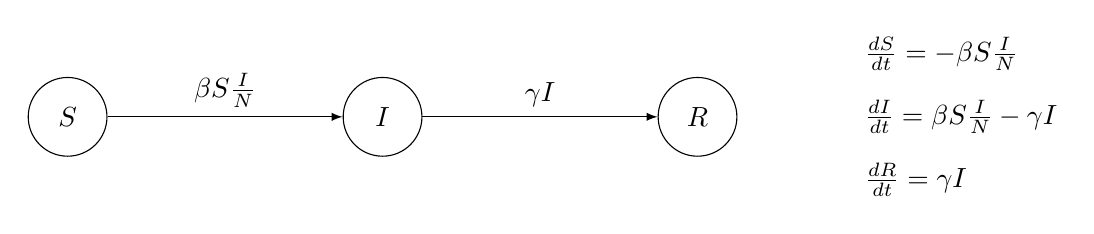
\begin{tikzpicture}
			\node[circle, draw, inner sep=0pt, minimum size=1cm] (S) at (0,0) {$S$};
			\node[circle, draw, inner sep=0pt, minimum size=1cm] (I) at (4,0) {$I$};
			\node[circle, draw, inner sep=0pt, minimum size=1cm] (R) at (8,0) {$R$};
			
			\draw[->,>=latex] (S) edge node[above] { $\beta S \frac{I}{N}$} (I);
			\draw[->,>=latex] (I) edge node[above] { $\gamma I$} (R);
			
			\node[anchor=west] at (10,.8) {$	\frac{dS}{dt} = - \beta S \frac{I}{N}$};
			\node[anchor=west] at (10,0) {$	\frac{dI}{dt} = \beta S \frac{I}{N} - \gamma I $};
			\node[anchor=west] at (10,-.8) {$\frac{dR}{dt} = \gamma I $};
		\end{tikzpicture}
	}
	\end{figure}
}

\frame{
	\frametitle{The SIR model}
	
		\begin{figure}
		\centering
		\scalebox{.8}{
			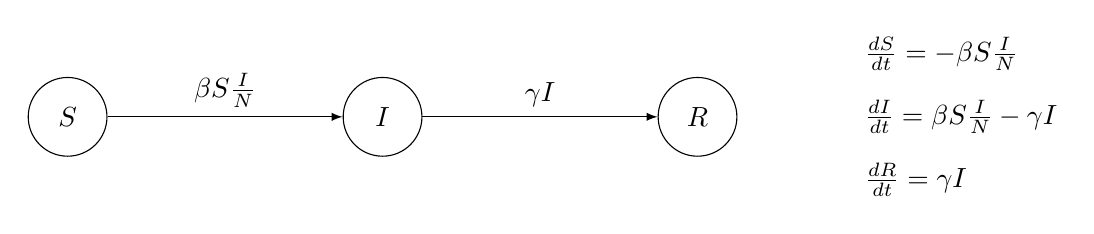
\begin{tikzpicture}
				\node[circle, draw, inner sep=0pt, minimum size=1cm] (S) at (0,0) {$S$};
				\node[circle, draw, inner sep=0pt, minimum size=1cm] (I) at (4,0) {$I$};
				\node[circle, draw, inner sep=0pt, minimum size=1cm] (R) at (8,0) {$R$};
				
				\draw[->,>=latex] (S) edge node[above] { $\beta S \frac{I}{N}$} (I);
				\draw[->,>=latex] (I) edge node[above] { $\gamma I$} (R);
				
				\node[anchor=west] at (10,.8) {$	\frac{dS}{dt} = - \beta S \frac{I}{N}$};
				\node[anchor=west] at (10,0) {$	\frac{dI}{dt} = \beta S \frac{I}{N} - \gamma I $};
				\node[anchor=west] at (10,-.8) {$\frac{dR}{dt} = \gamma I $};
			\end{tikzpicture}
		}
	\end{figure}
	Where:
	\begin{itemize}
		\item $S(t)$ is the number of people \alert{susceptible} to infection
		\item $I(t)$ is the number of people \alert{infected} (i.e. the prevalence)
		\item $R(t)$ is the number of people \alert{recovered} (lifelong immunity)
		\item $N$ is the population size ($S(t)+I(t)+R(t)=N$ for any $t$)
		\item $\beta$ is the \alert{infectious contact rate} (per day per person)
		\item $\gamma$ is the \alert{recovery rate} (1/infectious period)
	\end{itemize}
}

\frame{
	\frametitle{The SIR model}
	
	\begin{figure}
		\centering
		\scalebox{.8}{
			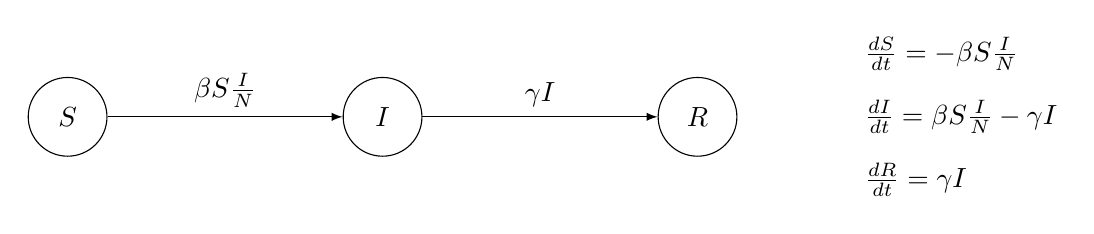
\begin{tikzpicture}
				\node[circle, draw, inner sep=0pt, minimum size=1cm] (S) at (0,0) {$S$};
				\node[circle, draw, inner sep=0pt, minimum size=1cm] (I) at (4,0) {$I$};
				\node[circle, draw, inner sep=0pt, minimum size=1cm] (R) at (8,0) {$R$};
				
				\draw[->,>=latex] (S) edge node[above] { $\beta S \frac{I}{N}$} (I);
				\draw[->,>=latex] (I) edge node[above] { $\gamma I$} (R);
				
				\node[anchor=west] at (10,.8) {$	\frac{dS}{dt} = - \beta S \frac{I}{N}$};
				\node[anchor=west] at (10,0) {$	\frac{dI}{dt} = \beta S \frac{I}{N} - \gamma I $};
				\node[anchor=west] at (10,-.8) {$\frac{dR}{dt} = \gamma I $};
			\end{tikzpicture}
		}
	\end{figure}
	\alert{Intuition} behind the SIR model:
	\begin{itemize}
		\item $I(t)/N$ is the proportion of infected (and infectious)
		\item $\beta I(t)/N$ is the daily number of contacts with infectious people
		\item hence each day, $\beta S I(t)/N$ people become infected (the \alert{force of infection})
	\end{itemize}
}

\frame{
	\frametitle{The SIR model}
	
	\begin{figure}
		\centering
		\scalebox{.8}{
			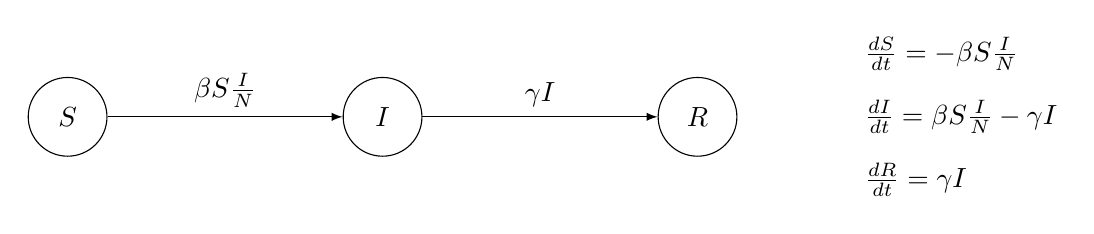
\begin{tikzpicture}
				\node[circle, draw, inner sep=0pt, minimum size=1cm] (S) at (0,0) {$S$};
				\node[circle, draw, inner sep=0pt, minimum size=1cm] (I) at (4,0) {$I$};
				\node[circle, draw, inner sep=0pt, minimum size=1cm] (R) at (8,0) {$R$};
				
				\draw[->,>=latex] (S) edge node[above] { $\beta S \frac{I}{N}$} (I);
				\draw[->,>=latex] (I) edge node[above] { $\gamma I$} (R);
				
				\node[anchor=west] at (10,.8) {$	\frac{dS}{dt} = - \beta S \frac{I}{N}$};
				\node[anchor=west] at (10,0) {$	\frac{dI}{dt} = \beta S \frac{I}{N} - \gamma I $};
				\node[anchor=west] at (10,-.8) {$\frac{dR}{dt} = \gamma I $};
			\end{tikzpicture}
		}
	\end{figure}
	\alert{Assumptions} behind the SIR model:
	\begin{itemize}
		\item homogeneous mixing
		\item $\beta$ and $\gamma$ constant over time
		\item all infections are observed
		\item no incubation, exponentially-distributed recovery
		\item lifelong immunity
		\item stable population
	\end{itemize}
}


\frame{
	\frametitle{Simulate a SIR in \texttt{R}}
	
	\begin{itemize}
		\item load library \texttt{deSolve} (and \texttt{tidyverse})
		\item set compartments and differential equations
	\end{itemize}
	\begin{figure}
		\centering
		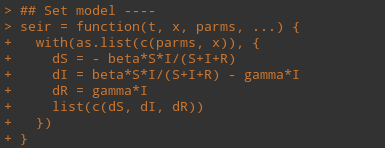
\includegraphics[width=0.55\linewidth]{simple_sir/simsir3.png}
	\end{figure}
	\pause
	\begin{itemize}
		\item set (fixed) values for parameters:	
		$\beta=0.8$; $\gamma=1/7$
	\end{itemize}
	\begin{figure}
		\centering
		
\includegraphics[width=0.55\linewidth]{simple_sir/simsir1.png}
	\end{figure}
\pause
	\begin{itemize}
	\item set (fixed) values for initial values
\end{itemize}
\begin{figure}
	\centering
	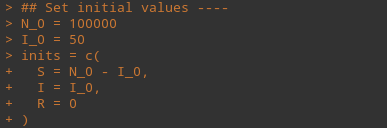
\includegraphics[width=0.55\linewidth]{simple_sir/simsir2.png}
\end{figure}
}


\frame{
	\frametitle{Simulate a SIR in \texttt{R}}
	\begin{itemize}
		\item solve the ODE system numerically (Runge-Kutta 4th order) to obtain unique solutions for $S(t)$, $I(t)$ and $R(t)$
	\end{itemize}
	$$
f(\beta,\gamma,S_0,I_0,R_0) = \{S(t),I(t),R(t)\}
$$
	\begin{figure}
		\centering
		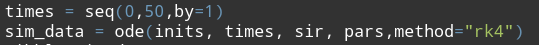
\includegraphics[width=0.65\linewidth]{simple_sir/simsir4.png}

	\end{figure}
	\begin{figure}
	\centering

	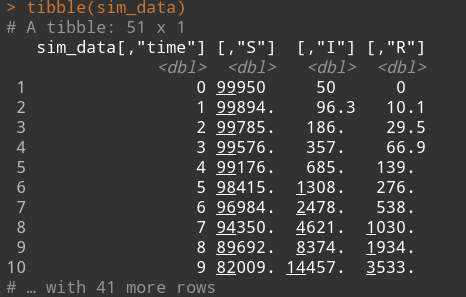
\includegraphics[width=0.65\linewidth]{simple_sir/simsir5.png}
\end{figure}

}

\frame{
	\frametitle{Simulate a SIR in \texttt{R}}

	\begin{figure}
		\centering
		\only<1>{
			with $\beta=0.8$; $\gamma=1/7$; $S_0=100000-50$; $I_0=50$ and $R_0=0$ \\ \bigskip
			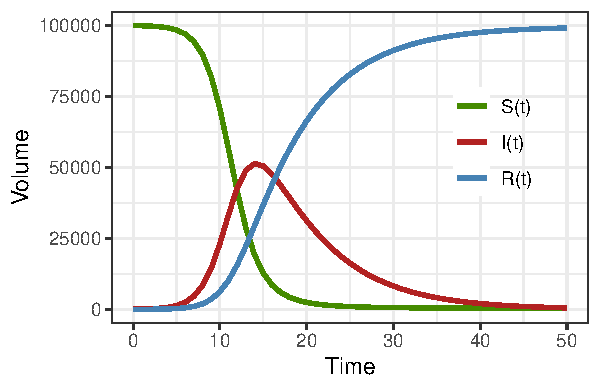
\includegraphics[width=0.7\linewidth]{simple_sir/example_sir1.pdf}
		}
		\only<2>{
			with $\beta = 1.1$ instead of $0.8$, we get \\ \bigskip
			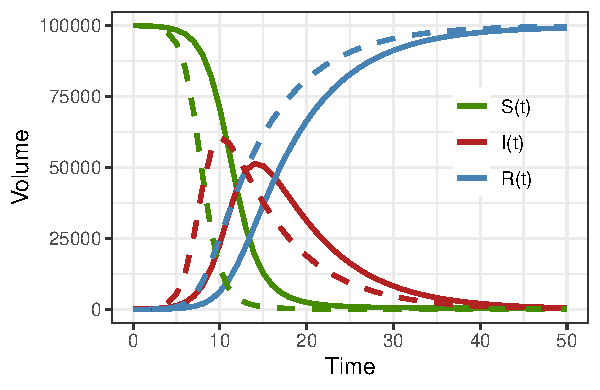
\includegraphics[width=0.7\linewidth]{simple_sir/example_sir2.pdf}
		}
		\only<3>{
			with $\beta = 0.6$ instead of $0.8$, we get \\ \bigskip
			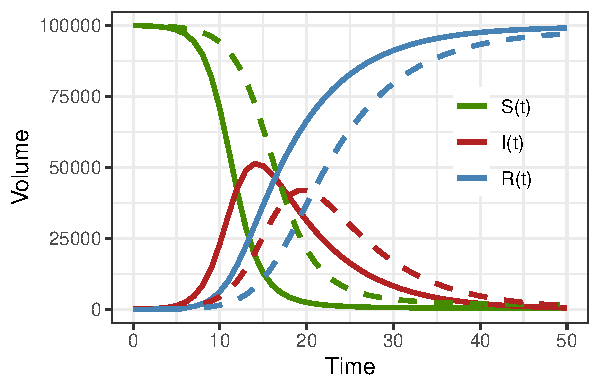
\includegraphics[width=0.7\linewidth]{simple_sir/example_sir3.pdf}
		}
		\only<4>{
		with $\gamma = 1/14$ instead of $1/7$, we get \\ \bigskip
		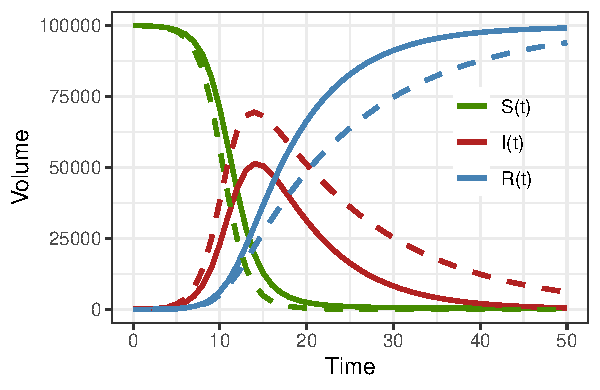
\includegraphics[width=0.7\linewidth]{simple_sir/example_sir4.pdf}
		}
		\only<5>{
		with $\gamma = 1/4$ instead of $1/7$, we get \\ \bigskip
		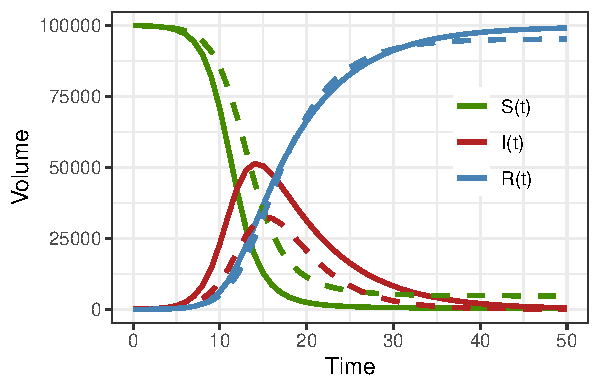
\includegraphics[width=0.7\linewidth]{simple_sir/example_sir5.pdf}
		}
		\only<6>{
		with $I(0) = 500$ instead of $50$, we get \\ \bigskip
		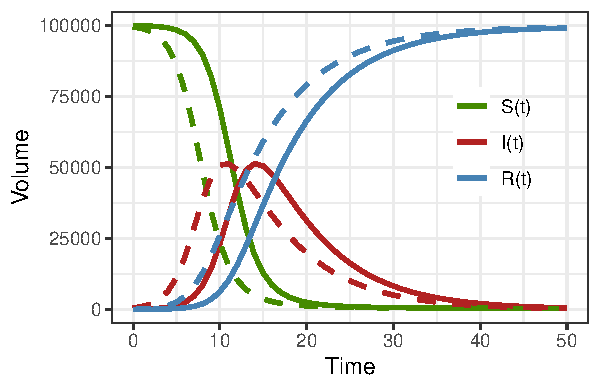
\includegraphics[width=0.7\linewidth]{simple_sir/example_sir6.pdf}
		}
		\only<7>{
		with $I(0) = 5$ instead of $50$, we get \\ \bigskip
		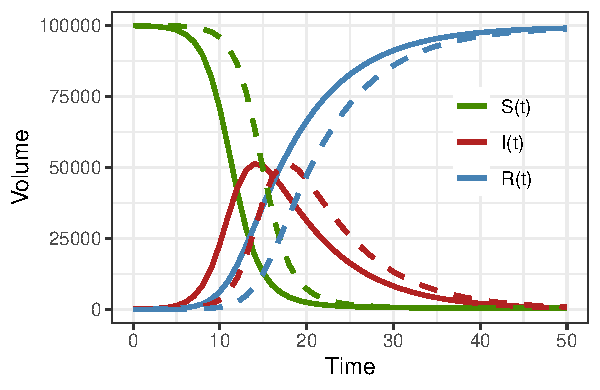
\includegraphics[width=0.7\linewidth]{simple_sir/example_sir7.pdf}
		}
		\only<8>{
		with $R(0) = 20,000$ instead of $0$, we get \\ \bigskip
		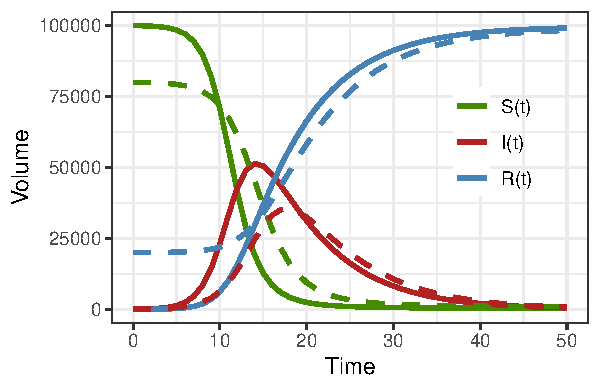
\includegraphics[width=0.7\linewidth]{simple_sir/example_sir8.pdf}
		}
	\end{figure}
}

\frame{
	\frametitle{Applications}
	Compartmental models have many uses:
	\begin{itemize}
		\item get \alert{mechanistic insight} about an epidemic (transmissibility levels, drivers of transmission)
		$$
		\mathcal{R}_0 = \frac{\beta}{\gamma}
		$$
		
		\item formalize and put numerical values on \alert{general concepts} \\ (herd immunity threshold...)
		$$
		V_c = \frac{1}{\mathcal R_0}
		$$
		
		\item produce (short-term) \alert{forecasts} accounting for contagion and immunity
	\end{itemize}
	
	\pause\vspace{2em}
	$\rightarrow$ all these uses are based on \alert{numerical values} for $\beta$, $\gamma$ and the initial conditions and their \alert{uncertainty}
}

\frame{
	\frametitle{Applications}
	Enters \alert{Bayesian inference}:
	\begin{itemize}
		\item infer parameter values by \alert{integrating data and domain knowledge}
		\item more efficient for complex models (high dimensionality)
		\item rigorously quantify and propagate uncertainty in parameter estimates and forecast
	\end{itemize}
	
	\pause\vspace{2em}
	$\rightarrow$ Markov Chain Monte Carlo (MCMC) methods and \alert{Stan}
}

\section{Bayesian inference with Stan}

\frame{
	\frametitle{Bayesian inference}
   $$\underbrace{p(\theta|y)}_{\text{posterior}} \propto \underbrace{p(y| \theta)}_{\text{likelihood}} \underbrace{p(\theta)}_{\text{prior}}$$
}

\frame{
	\frametitle{General principle}
	General principle of Bayesian inference:
	\begin{itemize}
		\item specify a complete Bayesian model
		\begin{itemize}
			\item[-] consider data $y = \{y_1,...,y_n\}$ and parameter $\theta$
			\item[-] specify an \alert{observation model, e.g.} $$p(y|\theta) = \prod_n \text{normal}(y_n | \theta,1)$$
			\item[-] complete the model with a \alert{prior distribution, e.g.} $$p(\theta) = \text{normal}(0,1)$$
		\end{itemize}
%		\item estimate the \alert{posterior distribution of $\theta$} 
%		$$ \Pr(\theta|y) = \frac{\Pr(y|\theta) \Pr(\theta)}{\Pr(y)}  $$
		\item sample the \alert{posterior distribution} of the parameter
	\end{itemize}
}



\frame{
	\frametitle{Stan}
	Stan is a probabilistic programming framework for Bayesian inference
	\begin{itemize}
		\item it is designed to let the user \alert{focus on modeling} while inference happens under the hood
		\item object-oriented language (based on \texttt{C++}) that supports many  operations, probability densities and ODE solvers
		\item extremely \alert{efficient} MCMC algorithm (Hamiltonian Monte Carlo)
		\item \alert{diagnostic tools} to evaluate the inference
		\item interfaces in \texttt{R} (package \texttt{rstan}), \texttt{python}, \texttt{julia}...	
	\end{itemize}
}



\frame{
	\frametitle{Stan program structure}
	A Stan program is structured in \alert{blocks}:
	\begin{itemize}
	    \item  \texttt{functions} 
		\item  \texttt{data} 
		\item  \texttt{transformed data} 
		\item  \texttt{parameters} 
		\item  \texttt{transformed parameters} 
		\item  \texttt{model} 
        \item  \texttt{generated quantities} 
	\end{itemize}
}

\frame{
	\frametitle{Stan example}
	\begin{itemize}
		\item the \texttt{data} block defines data variables
		\begin{figure}
			\centering
			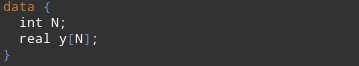
\includegraphics[width=0.6\linewidth]{example_linear/example_linear1.png}
		\end{figure}
		
		\item the \texttt{parameters} block defines parameters
		\begin{figure}
			\centering
			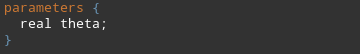
\includegraphics[width=0.6\linewidth]{example_linear/example_linear2.png}
		\end{figure}
		
		\item the \texttt{model} block defines the \alert{target log probability density function}
		\begin{figure}
			\centering
			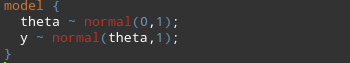
\includegraphics[width=0.6\linewidth]{example_linear/example_linear3.png}
		\end{figure}
		\item save in \texttt{model\_linear.stan}
	
	\end{itemize}
}


\frame{
	\frametitle{Stan example}
	We then explore the target with Stan's MCMC \alert{sampler}:
	\begin{itemize}
		\item load \texttt{rstan} package
		\begin{figure}
			\centering
			
\includegraphics[width=0.7\linewidth]{example_linear/run_stan1.png}
		\end{figure}
		
		\item simulate $N=50$ data points with $\theta=0.7$
		\begin{figure}
			\centering
			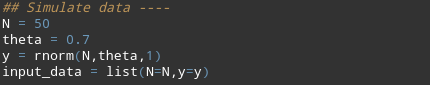
\includegraphics[width=0.7\linewidth]{example_linear/run_stan2.png}
		\end{figure}
		
		\item run MCMC sampling
		\begin{figure}
			\centering
			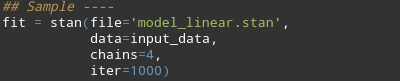
\includegraphics[width=0.7\linewidth]{example_linear/run_stan3.png}
		\end{figure}
	\end{itemize}
}

\frame{
	\frametitle{Stan example}
	We use \alert{multiple chains} and inspect convergence after warm-up
	\begin{figure}
		\centering
		\only<1>{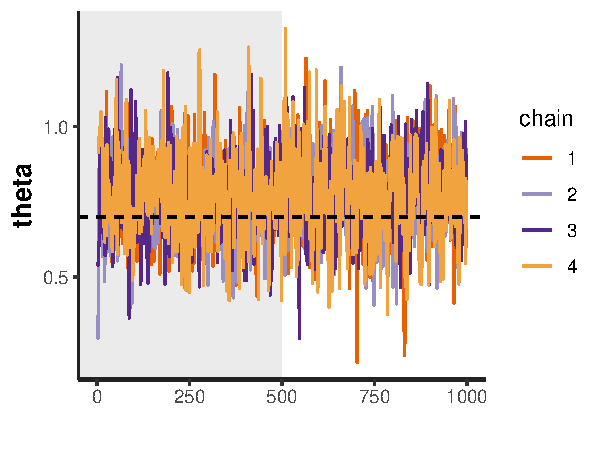
\includegraphics[width=.6\linewidth]{example_linear/trace_theta.pdf}}
		\only<2>{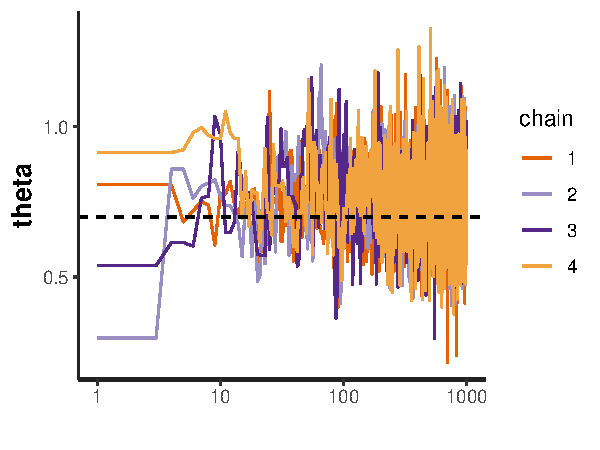
\includegraphics[width=.6\linewidth]{example_linear/trace_theta_init.pdf}}
	\end{figure}
}

\frame{
	\frametitle{Stan example}
	The post-warm-up samples of $\theta$ approximate its \alert{posterior distribution}
	\begin{figure}
		\centering
		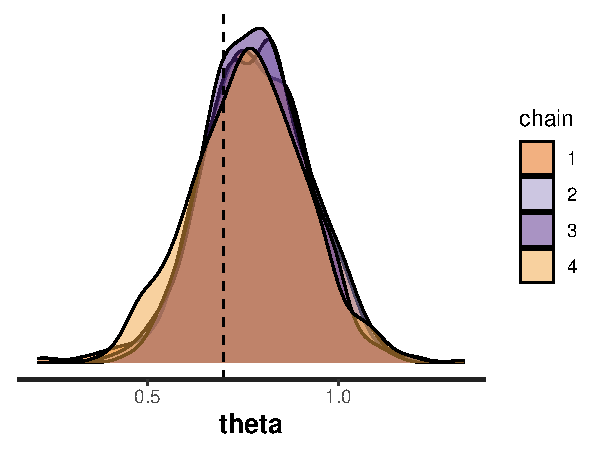
\includegraphics[width=.6\linewidth]{example_linear/post_theta.pdf}
	\end{figure}
}

%\frame{
%	\frametitle{Stan example}
	
%	We run \alert{basic diagnostics tools}: divergences, tree depth, energy
%		\begin{figure}
%			\centering
%			\vspace{1em}
%			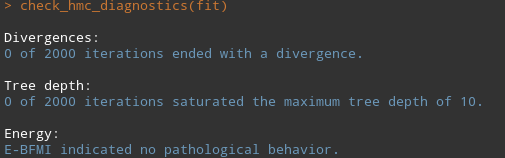
\includegraphics[width=.8\linewidth]{example_linear/run_stan5.png}
%		\end{figure}

%}

\frame{
	\frametitle{Stan example}
	
	Printing the object gives:
	\begin{itemize}
		\item \alert{diagnostics}: effective sample size, Gelman-Rubin $\hat{R}$
		\item \alert{inference}: full posterior distribution of $\theta$
	\begin{figure}
		\centering
		\vspace{1em}
		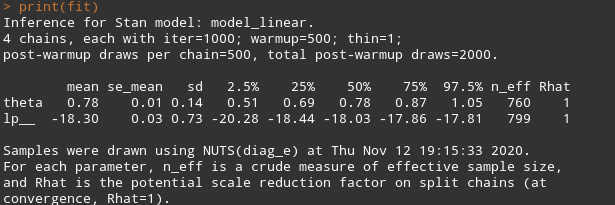
\includegraphics[width=1\linewidth]{example_linear/run_stan4.png}
	\end{figure}
	\end{itemize}
}

\section{Fitting a simple SIR}


\frame{
	\frametitle{Example dataset}
	Outbreak of influenza A (H1N1) at a \alert{British boarding school} in 1978 (available in \texttt{R} package \texttt{outbreaks})
	\begin{itemize}
		\item 763 students, 512 had symptoms
		\item daily number of students in bed over 14 days (\alert{prevalence})
		\begin{figure}
			\centering
			\vspace{.5em}
			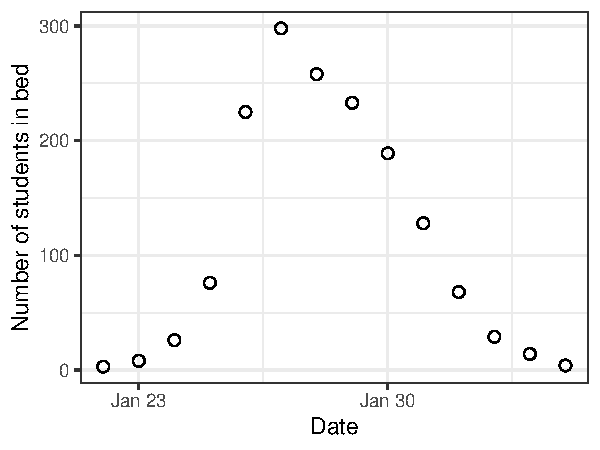
\includegraphics[width=.6\linewidth]{boarding_school/inbed.pdf}
		\end{figure}
	\end{itemize}	
}

\frame{
	\frametitle{Specify the model}
	Points to consider:
	\begin{itemize}
		\item prevalence data: $\mathds{I}_{t}$ with $t \in \{1,\ldots,14\}$
		\item inputs that will remain fixed: $\{S_0=762,I_0=1,R_0=0\}$
		\item map data $\mathds{I}_{t}$ to SIR model output $I(t)$ using an observation model  with an appropriate \alert{probability distribution}:
		$$
		p(\mathds{I}|\theta) = \prod_{t=1}^{14} \text{NegBinomial}(\mathds{I}_{t} | I(t), \phi)
		$$
		\item parameters to estimate: $\theta = \{\beta,\gamma,\phi\}$
		\item \alert{prior distributions} 
		\vspace{-1em}
		$$p(\beta) = \text{Exponential}(1)$$
		$$p(1/\gamma) = \text{Normal}^+(2,0.5)$$
		$$p(1/\phi) = \text{Exponential}(5)$$
	\end{itemize}
}

\frame{
	\frametitle{Code the model}
	\faWarning\ Note that further we are using ODE signature as presented in the paper. Since then a new interface has become available.
}


\frame{
	\frametitle{Code the model}
	We define the ODE system in the \texttt{function} block
		\begin{figure}
			\centering
			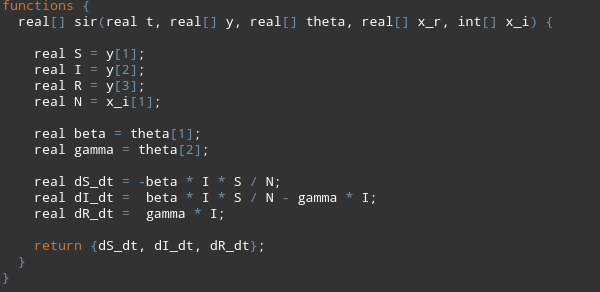
\includegraphics[width=1\linewidth]{boarding_school/stan_code1.png}
		\end{figure}
	\faWarning\ Be careful of the signature and formats!
}

\frame{
	\frametitle{Code the model}
	We declare the data variables in the \texttt{data} block
		\begin{figure}
			\centering
			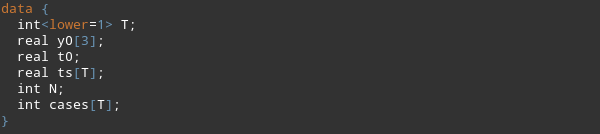
\includegraphics[width=1\linewidth]{boarding_school/stan_code2.png}
		\end{figure}
	
	\pause
	and define additional data variables in \texttt{transformed data} block
	\begin{figure}
		\centering
		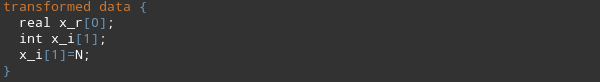
\includegraphics[width=1\linewidth]{boarding_school/stan_code3.png}
	\end{figure}
}

\frame{
	\frametitle{Code the model}
	Similarly, parameters are declared in the \texttt{parameters} block
		\begin{figure}
			\centering
			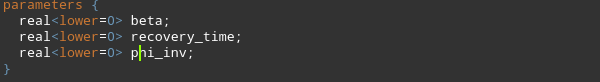
\includegraphics[width=1\linewidth]{boarding_school/stan_code4.png}
		\end{figure}
	\faWarning\ It sometimes makes more sense to transform some parameters (e.g., recovery rate $\gamma$ and overdispersion $\phi$) to improve interpretability
	}

\frame{
	\frametitle{Code the model}
	In \texttt{transformed parameters}, we define additional parameters and solve the ODE system
		\begin{figure}
			\centering
			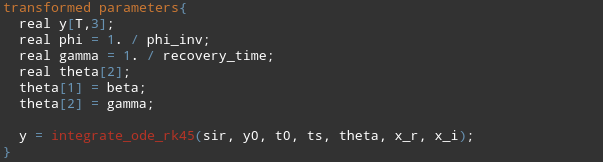
\includegraphics[width=1\linewidth]{boarding_school/stan_code5.png}
		\end{figure}
}


\frame{
	\frametitle{Code the model}
	\begin{figure}
		\centering
		
\includegraphics[width=.8\linewidth]{boarding_school/stan_code5bis.png}
	\end{figure}
	\begin{itemize}
	\item Be careful about the \alert{formats and signatures}
	\begin{itemize}
			\item[-] the ODE output \texttt{y} is an array of size \texttt{T}$\times$3 (number of time steps and number of compartments)
			\item[-] \texttt{sir} is the name of the function defined in the \texttt{function} block
			\item[-] \texttt{y0} is an array of size 3 defined in the \texttt{data} block
			\item[-] \texttt{ts} is an array of size \texttt{T} defined in the \texttt{data} block
			\item[-] \texttt{theta} is an array of size 2 storing the parameters
			\item[-] \texttt{x\_r} is defined as empty in \texttt{transformed data}, but can be used to store fixed real values
			\item[-] \texttt{x\_i} is an array of size 1 storing the population size \texttt{N} (can also be used to store fixed integer values)
	\end{itemize}
	\end{itemize}
}
\frame{
	\frametitle{Code the model}
	\begin{figure}
		\centering
		
\includegraphics[width=.8\linewidth]{boarding_school/stan_code5bis.png}
	\end{figure}
	\begin{itemize}
		\item Chose an ODE solver. In the previous interface:
	\begin{itemize}
		\item[-] \texttt{integrate\_ode\_rk45} uses the Runge-Kutta method (quicker but non-adapted to stiff systems)
		\item[-] \texttt{integrate\_ode\_bdf} uses the backward differentiation method (slower but adapted to stiff systems)
	\end{itemize}
	    \item In the new interface:
	\begin{itemize}
	    \item[-] \texttt{ode\_bdf}, \texttt{ode\_adams}, \texttt{ode\_rk45}, 
	    \item[-] \texttt{ode\_bdf\_tol},\texttt{ode\_adams\_tol}, \texttt{ode\_rk45\_tol}
	\end{itemize}
	\end{itemize}
}

\frame{
	\frametitle{Code the model}
	In the \texttt{model} block, we write the priors and the observation model
	\begin{figure}
		\centering
		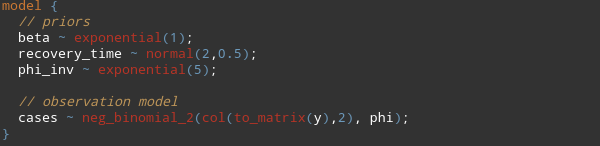
\includegraphics[width=1\linewidth]{boarding_school/stan_code6.png}
	\end{figure}
	\faWarning\ It's important that the chosen distributions correspond with the boundaries set in the \texttt{parameters} block (\texttt{<lower=0>})

\bigskip
	\faWarning\ \texttt{col(to\_matrix(y))} extracts the 2nd column of \texttt{y}
}


\frame{
	\frametitle{Code the model}
	Last, we add a \texttt{generated quantities} block that does not influence sampling and can be used for ``post-processing'':
	\begin{itemize}
		\item reproduction number $\mathcal{R}_0 = \beta/\gamma$
		\item model predictions of prevalence from the negative binomial
	\end{itemize}

	\begin{figure}
		\centering
		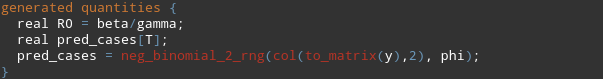
\includegraphics[width=1\linewidth]{boarding_school/stan_code7.png}
	\end{figure}
}

\frame{
	\frametitle{Code the model}
	In summary:
	\begin{itemize}
		\item \texttt{functions}: define the ODE system (\faWarning\ signature and formats)
		\item \texttt{data}: declare data variables that will be provided
		\item \texttt{tranformed data}: additional quantities that can be computed internally or from \texttt{data} variables 
		\item \texttt{parameters}: declare parameters (\faWarning\ boundaries)
		\item \texttt{transformed parameters}: quantities that can be computed internally or from \texttt{data} or \texttt{parameters} variables,
		including the ODE output (\faWarning \ signature and format)
		\item \texttt{model}: priors and observation model
		\item \texttt{generated quantities}: additional quantities that can be computed without influencing the sampling
	\end{itemize}

}


\frame{
	\frametitle{Inference}
	As before, we conduct the inference from \texttt{R} with the package \texttt{rstan}:
	\begin{figure}
		\centering
		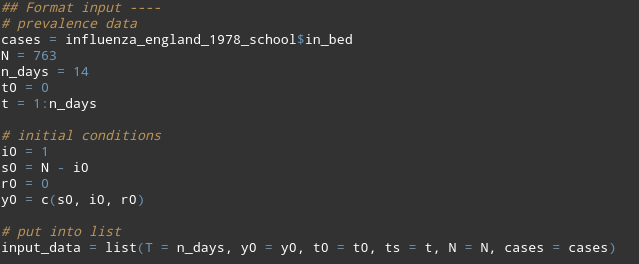
\includegraphics[width=1\linewidth]{boarding_school/r_code1.png}
	\end{figure}

	\faWarning\ data is put in a list with names matching the \texttt{data} block in Stan
}

\frame{
	\frametitle{Inference}
	Hit the inference button!
	\begin{figure}
		\centering
		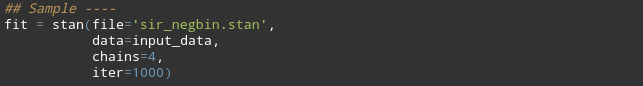
\includegraphics[width=1\linewidth]{boarding_school/r_code2.png}
	\end{figure}
}

\frame{
	\frametitle{Diagnostics}
	Use the basic diagnostics tools:
	\begin{figure}
		\centering
		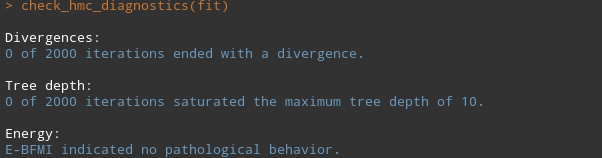
\includegraphics[width=1\linewidth]{boarding_school/r_code3.png}
	\end{figure}
}

\frame{
	\frametitle{Diagnostics}
	Examine trace plots:
	\begin{figure}
		\centering
		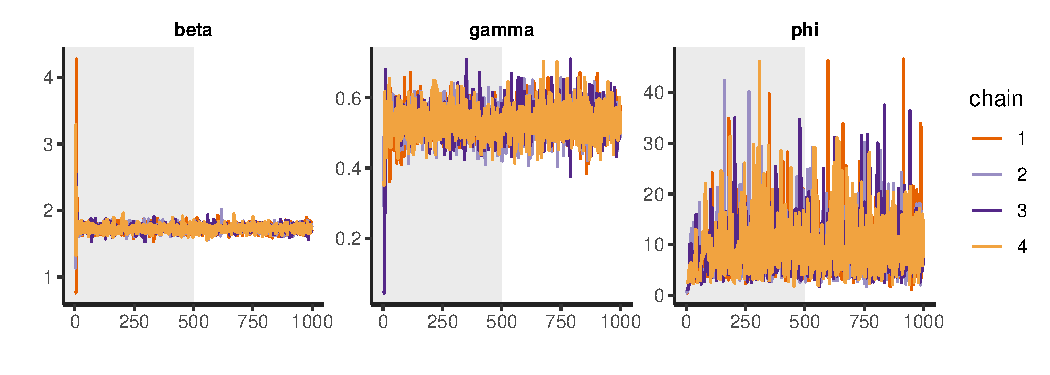
\includegraphics[width=1\linewidth]{boarding_school/trace_theta.pdf}
	\end{figure}
}

\frame{
	\frametitle{Diagnostics}
	Examine chain mixing:
	\begin{figure}
		\centering
		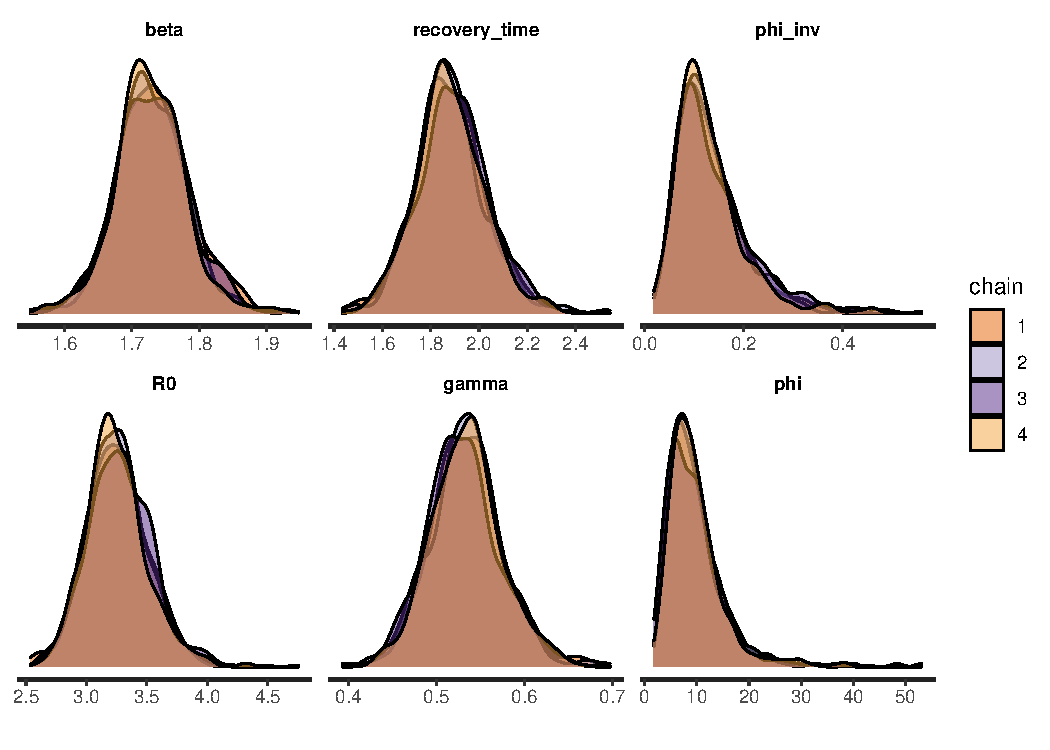
\includegraphics[width=.8\linewidth]{boarding_school/post_theta.pdf}
	\end{figure}
}

\frame{
	\frametitle{Diagnostics}
	Posterior predictive checking:
	\begin{figure}
		\centering
		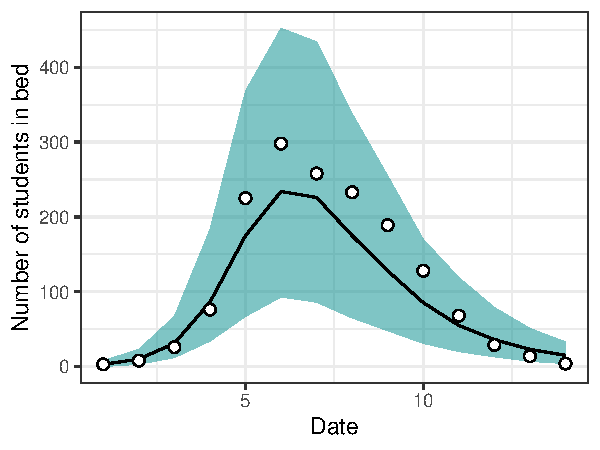
\includegraphics[width=.6\linewidth]{boarding_school/inbed_fit.pdf}
	\end{figure}
}

\frame{
	\frametitle{Results}
	Print the results:
	\begin{figure}
		\centering
		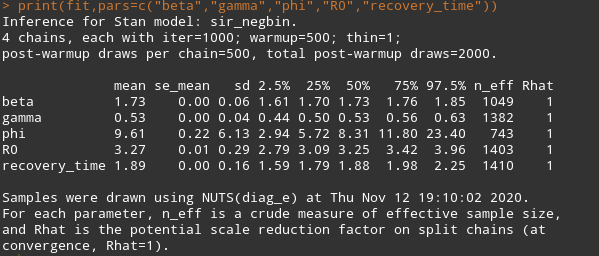
\includegraphics[width=1\linewidth]{boarding_school/r_code4.png}
	\end{figure}
}

\frame{
	\frametitle{Results}
	\begin{itemize}
		\item we estimate $\mathcal{R}_0$ to 3.3 (95\% credible interval: 2.8 to 4.0)
		%\item this corresponds to the direct estimation from the final size of the epidemic %$q = 512/763 = 0.67$
		%\vspace{-.5em}
		%$$
		%\mathcal{R}_0 = 1 / (1-q) = 3.03
		%$$
		\item based on \alert{many assumptions}:
		\begin{itemize}
			\item[-] common to all SIRs (homogeneous mixing, no incubation...)
			\item[-] prior distributions (especially on the recovery period)
			\item[-] complete ascertainment, no asymptomatics
			\item[-] no initial immunity
		\end{itemize}
	\end{itemize}
		
}


\section{Bayesian workflow}

\frame{
	\frametitle{Box's loop}
	In practice, the situation is often less clear than in the boarding school example:
	\begin{itemize}
		\item[-] incomplete data, insufficient domain knowledge
		\item[-] uncertainty on \alert{necessary model features}
	\end{itemize}	
}


\frame{
	\frametitle{Box's loop}
	\begin{figure}
		\centering
		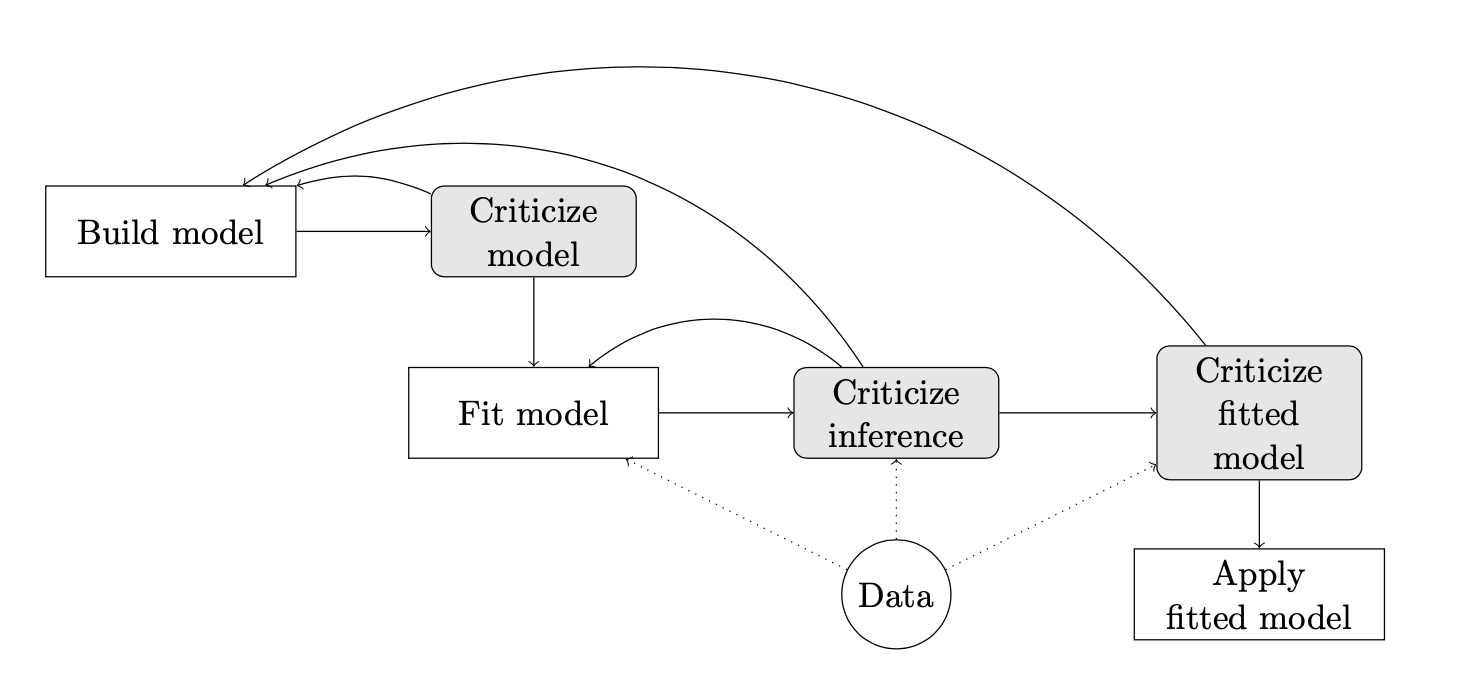
\includegraphics[width=.8\linewidth]{boarding_school/Boxes_loop.png}
	\end{figure}
}

\frame{
	\frametitle{Model development}
	Model development is an iterative procedure:
	\begin{itemize}
		\item[-] troubleshoot the model before fitting it,
		\item[-] criticize the inference after attempting a fit,
		\item[-] criticize the fitted model.
	\end{itemize}
}

\section{Using simulations to understand the model}

\frame{
	\frametitle{Model development}
	\alert{Fake data} can be used to probe the model and better understand its behaviour:
	\begin{itemize}
		\item[-] prior predictive checks
		\item[-] simulation study
	\end{itemize}	
}

\frame{
	\frametitle{Prior predictive checks}
	\alert{Prior predictive checking} consists in simulating data from the priors:
	\begin{itemize}
		\item visualize priors (especially after transformation)
		\item this shows the range of data compatible with the model
		\item it helps understand the \alert{adequacy of the chosen priors}, as it is often easier to elicit expert knowledge on measureable quantities of interest rather than abstract parameter values
		\bigskip\pause
		\item remove (or switch off) the likelihood from the \texttt{model} block
	\end{itemize}
	\begin{figure}
		\centering
		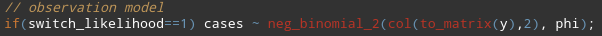
\includegraphics[width=1\linewidth]{boarding_school/stan_code6bis.png}
	\end{figure}
}

\frame{
	\frametitle{Prior predictive checks}
	Simulating priors in the boarding school example:
	\begin{figure}
		\centering
		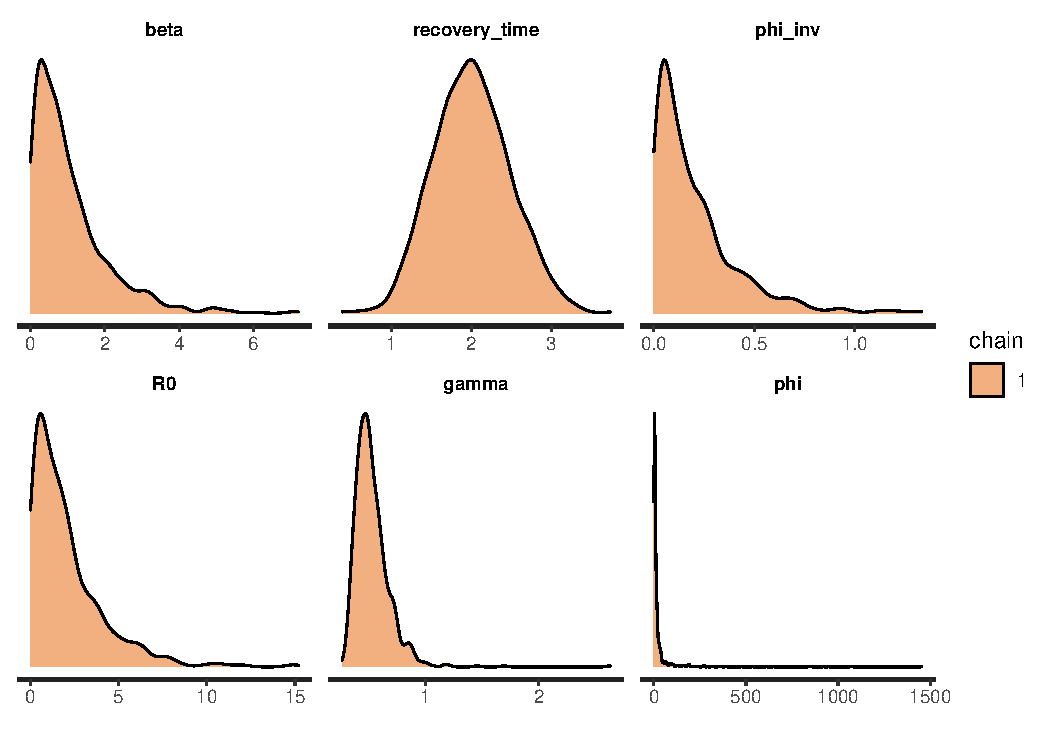
\includegraphics[width=.8\linewidth]{boarding_school/prior_theta.pdf}
	\end{figure}
}

\frame{
	\frametitle{Prior predictive checks}
	Prior predictive check: simulating potential \alert{epidemic trajectories}
	\begin{figure}
		\centering
		\only<1>{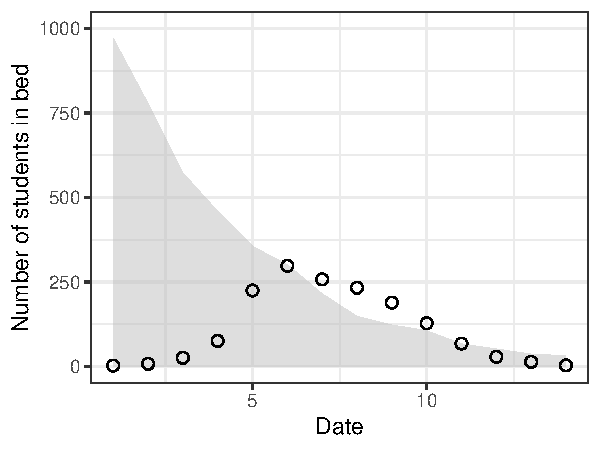
\includegraphics[width=.6\linewidth]{boarding_school/inbed_fit_prior.pdf}}
		\only<2>{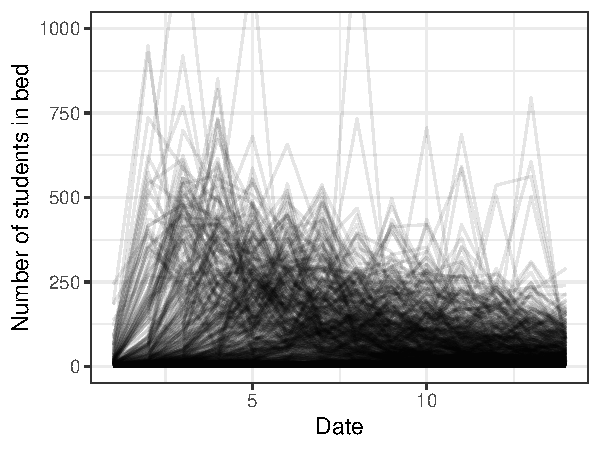
\includegraphics[width=.6\linewidth]{boarding_school/inbed_fit_prior_traj.pdf}}
	\end{figure}
}

\frame{
	\frametitle{Prior predictive checks}
	Prior predictive checks bring insight about \alert{non-obvious features}:
	\begin{itemize}
		\item even if the priors seem weakly informative, there is actually not a lot of leeway
		\item \alert{highly constrained} model: 
		\begin{itemize}
		\item[-] if $\beta$ is high, the epidemic will stop rapidly by lack of susceptibles
		\item[-] if $\beta$ is small, the epidemic will be small
	\end{itemize}
	\item the negative binomial distribution might lead to problems in extreme situations, e.g. more cases ($>$1000) than the overall number of students
	\end{itemize}
}

\frame{
	\frametitle{Simulation-based checks}
	A \alert{simulation study} consists out of two steps:
	\begin{itemize}
		\item simulate data with specified parameter values
		\item measure the capacity of the model to recover the chosen parameter values
\end{itemize}
	\bigskip\pause
	Many advantages:
	\begin{itemize}
	\item check for bugs and coding mistakes
	\item check for \alert{identifiability} issues
	\item compare different versions of a model
	\item understand in what \alert{situations} a model works or not
\end{itemize}
}

\frame{
	\frametitle{Simulation-based checks}
	Let's go back to the \alert{simple SIR example} from the beginning:
	\begin{itemize}
		\item set $\beta=2$ and $\gamma=0.5$ (so that $\mathcal{R}_0=4$) 
		\item simulate in a susceptible population of size $N=763$ with $I_0=1$
	\end{itemize}
	\begin{figure}
	\centering
	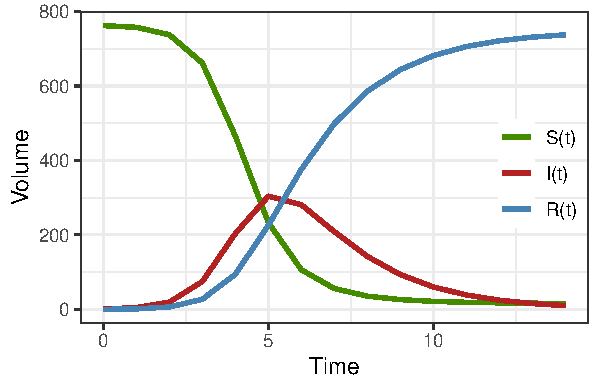
\includegraphics[width=.6\linewidth]{boarding_school/example_sir1.pdf}
\end{figure}
}

\frame{
	\frametitle{Simulation-based checks}
	Add noise with a \alert{negative binomial} distribution with $\phi=15$
	\begin{figure}
		\centering
		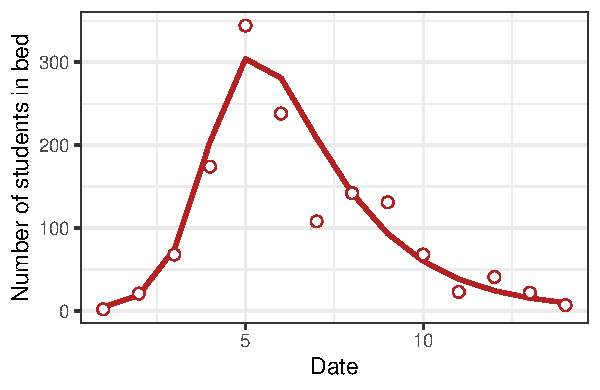
\includegraphics[width=.6\linewidth]{boarding_school/example_sir2.pdf}
	\end{figure}
}

\frame{
	\frametitle{Simulation-based checks}
	Fit the \alert{same model} as for the boarding school example
	\begin{figure}
		\centering
		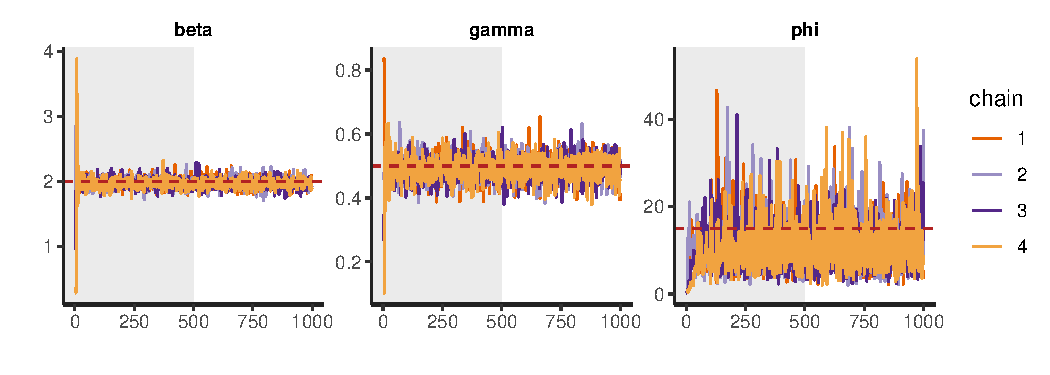
\includegraphics[width=1\linewidth]{boarding_school/trace_theta_sim.pdf}
	\end{figure}
}


\frame{
	\frametitle{Simulation-based checks}
	Posterior predictive checking
	\begin{figure}
		\centering
		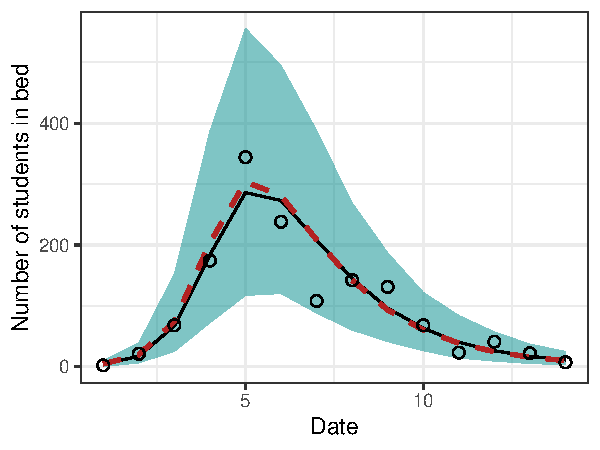
\includegraphics[width=.6\linewidth]{boarding_school/inbed_fit_sim.pdf}
	\end{figure}
}


\frame{
	\frametitle{Simulation-based checks}
	\bigskip
	Compare the posterior distributions of the parameters with the \alert{``truth''}
	\begin{figure}
		\centering
		\includegraphics[width=.9\linewidth]{boarding_school/post_theta_sim.pdf}
	\end{figure}
	\begin{itemize}
		\vspace{-1em}
	\item no identifiability issue
	\item $\beta$ and $\gamma$ are well estimated, but $\phi$ is not
	\item try with other values to understand \alert{when does the model break}
	\end{itemize}
}
%
%\section{Extension: Covid-19 transmission in Switzerland}
%
%\frame{
%
%	\frametitle{New Covid-19 cases in Switzerland in 2020}
%	\begin{figure}
%		\centering
%		\includegraphics[scale=0.8]{extension/swiss_data.png}
%	\end{figure}
%}
%
%\frame{
%    %TODO: priors
%    \frametitle{Basic SIR}
%    \textit{Transformed parameters} block
%    \vspace{-7mm}
%    \begin{center}
%     \includegraphics[scale=0.6]{extension/transformed_parameters_0.png}
%    \end{center}
%    \textit{Model} block
%    \vspace{-7mm}
%    \begin{figure}
%        \includegraphics[scale=0.6]{extension/model_0.png}
%    \end{figure}
%}
%
%
%\frame{
%    \frametitle{Basic SIR}
%    \begin{figure}
%		\centering
%		\includegraphics[scale=0.4]{extension/sir_diag.png}
%	\end{figure}
%	    \begin{figure}
%		\centering
%		\includegraphics[scale=0.13]{extension/swiss_fit1.png}
%	\end{figure}
%}
%
%\frame{
%    \frametitle{Adding underreporting: Stan code}
%    
%    \textit{parameters} block
%    \vspace{-7mm}
%    \begin{figure}
%        \centering
%        \includegraphics[scale=0.6]{extension/parameters_1.png}
%    \end{figure}
%    
%    \textit{transformed parameters} block
%    \vspace{-7mm}
%        \begin{figure}
%        \centering
%        \includegraphics[scale=0.6]{extension/transformed_parameters_1.png}
%    \end{figure}
%    
%    
%    \textit{model} block
%    \vspace{-7mm}
%    \begin{figure}
%        \centering
%        \includegraphics[scale=0.6]{extension/model_1.png}
%    \end{figure}
%}
%    
%\frame{
%    \frametitle{Adding underreporting: posterior predictive check}
%    \begin{figure}
%        \centering
%        \includegraphics[scale=0.2]{extension/underreporting.png}
%    \end{figure}
%}
%
%\frame{
%    \frametitle{Adding incubation time}
%    \begin{figure}
%        \includegraphics[scale=0.15]{extension/seir.jpeg}
%    \end{figure}
%    \begin{figure}
%        \centering
%        \includegraphics[0.6]{extension/seir_equations.png}
%    \end{figure}
%    Incubation time between 1/2 and 30 days $\rightarrow a \sim \mathcal{N}^+(0.4, 0.5)$
%}
%
%\frame{
%    \frametitle{Adding incubation time}
%    \begin{figure}
%        \centering
%        \includegraphics[scale=0.15]{extension/swiss_fit2.png}
%    \end{figure}
%}
%
%\frame{
%    \frametitle{Adding incubation time}
%    \begin{figure}
%        \centering
%        \includegraphics[scale=0.2]{extension/a_distrib.png}
%    \end{figure}
%        $\text{Domain knowledge} \rightarrow \frac{1}{a} \sim \mathcal{N}^+(6, 1)$
%}
%
%\frame{
%    \frametitle{Adding incubation time}
%    \begin{itemize}
%        \item P(reported) is very low ( $\leq$  1\%)
%        \vspace{2mm}
%        \item Indeed, in a SEIR model, cases only decrease through immunity
%        \vspace{2mm}
%        \item We need to model control measures
%    \end{itemize}
%}
%
%\frame{
%\frametitle{Modeling control measures}
%%TODO image of logistic function
%$\beta(t) = f(t) * \beta$, with $f(t) = \eta + (1 - \eta) * \frac{1}{1 + exp(\xi * (t - t_1 - \nu))}$
%\newline
%\textbf{Parameters}
%\begin{itemize}
%    \item $\eta$ is the decrease of transmission while control measures are fully in place
%    \item $\xi$ is the slope of the decrease
%    \item $\nu$ is the delay (after the date of introduction of control measures) until the measures are 50% effective
%\end{itemize}
%\textbf{Priors}
%\begin{itemize}
%    \item $\eta \sim \beta(2.5, 4)$ which means we expect governmental measures to reduce transmission, but not all the way to zero. 
%    \item $\nu \sim exponential(1/5)$ which means the delay should be around a week but could be lower or quite higher. 
%    \item $\xi \sim \mathcal{U}(0.5, 1.5)$, which means the slope has to be positive.
%\end{itemize}
%}
%
%\frame{
%    \frametitle{Modeling control measures}
%    \begin{figure}
%        \centering
%        \includegraphics[scale=0.22]{extension/pair_plot.png}
%    \end{figure}
%}
%
%\frame{
%    \frametitle{Using serological survey data}
%    Survey data from May 4 to May 7 in Geneva (83 / 775 have antibodies)
%    
%    \textbf{Assumptions:}
%    \begin{itemize}
%        \item Geneva is representative of Switzerland
%        \item Having antibodies = being in the R compartment
%    \end{itemize}
%    \vspace{2mm}
%    \textit{transformed parameters} block
%    \vspace{-7mm}
%    \begin{figure}
%        \hspace*{-0.9cm}
%        \includegraphics[scale=0.58]{extension/transformed_parameters_sero.png}
%    \end{figure}
%    \newline
%    \textit{model} block
%    \vspace{-7mm}
%    \begin{figure}
%         \hspace*{-0.9cm}
%        \includegraphics[scale=0.58]{extension/model_sero.png}
%    \end{figure}
%}
%
%
%\frame{
%    \frametitle{Final model}
%    \begin{figure}
%        \centering
%        \includegraphics[scale=0.10]{extension/swiss_fit4.png}
%    \end{figure}
%}
%
%\frame{
%\frametitle{Possible improvements}
%    \begin{itemize}
%        \item Relax assumptions
%        \item Incorporate testing or death data
%        \item Stratify by age, location...
%        \item ...
%    \end{itemize}
%}
%
%\frame{
%\frametitle{Extension conclusion}
%Building a model step by step using the Bayesian workflow allows us
%\begin{itemize}
%    \item to understand its failure modes better
%    \item to know when we need to add more information into the model
%    \item to be more transparent by sharing the different versions
%\end{itemize}
%
%}


\section{Conclusions}

\frame{
	\frametitle{Conclusions}
	General comments:
	\begin{itemize}
		\item develop models that correspond to the \alert{data-generating mechanisms}
		\item use Bayesian inference to \alert{propagate uncertainty} from the data (and priors) into the results (and forecasts)
		\item carefully examine the modelling process (Bayesian workflow)
		\item be transparent about assumptions (open code)
	\end{itemize}
	\bigskip 
	
	Try by yourself!
		\begin{itemize}
		\item \url{https://github.com/charlesm93/disease_transmission_workflow}
		\item julien.riou@ispm.unibe.ch
	\end{itemize}
}

\frame{
	\frametitle{Acknowledgements \& ressources}
	\begin{itemize}
		\item Michael Betancourt, \textit{Introduction to Stan} \\ \url{https://betanalpha.github.io/assets/case_studies/stan_intro.html}
		\item Andrew Gelman et al., \textit{Bayesian workflow} \\ \url{https://arxiv.org/abs/2011.01808}
		\item Chi Feng, \textit{MCMC interactive gallery} \\ \url{https://chi-feng.github.io/mcmc-demo/app.html}
		\item Daniel Lee, \textit{ODEs in Stan} \\ \url{https://youtu.be/hJ34_xJhYeY}
		\item Ben Bales, Sebastian Weber
, \textit{Upgrading to the new ODE interface} \\ \url{https://mc-stan.org/users/documentation/case-studies/convert_odes.html}
	\end{itemize}
}


\section{Bonus}

\frame{
	\frametitle{Example}
	Example with SARS-CoV-2 from \alert{Hauser et al.~(2020)}:
	\vspace{1em}
	
	\begin{figure}
		\centering
		\includegraphics[width=.9\linewidth]{example_hauser/paper_ref.png}
	\end{figure}
}


\frame{
	\frametitle{Example}
	In Hubei province (China):
	\begin{figure}
		\centering
				\includegraphics[width=.9\linewidth]{example_hauser/data_china.pdf}
	\end{figure}
}


\frame{
	\frametitle{Example}
	Specific features and natural history of SARS-CoV-2 infection:
	\begin{itemize}
		\item Incubation period of 5 days (S\alert{E}IR)
		\item Pre-symptomatic transmission accounting for 44-48\% (SE\alert{P}IR)
		\item Symptoms in 81\% (95\%CrI 71\%–89\%) of cases (SEPI\alert{A}R)
		\item Respiratory virus transmitted through contacts \\ (\alert{age stratification})
		\item Effect of control measures (\alert{time-dependent force of infection})
		\item Mortality is delayed by $20.2 \pm 11.6$ days (\alert{fit to mortality data})
	\end{itemize}
}

\frame{
	\frametitle{Example}
	 Final model:
	 \begin{figure}
	 \scalebox{.78}{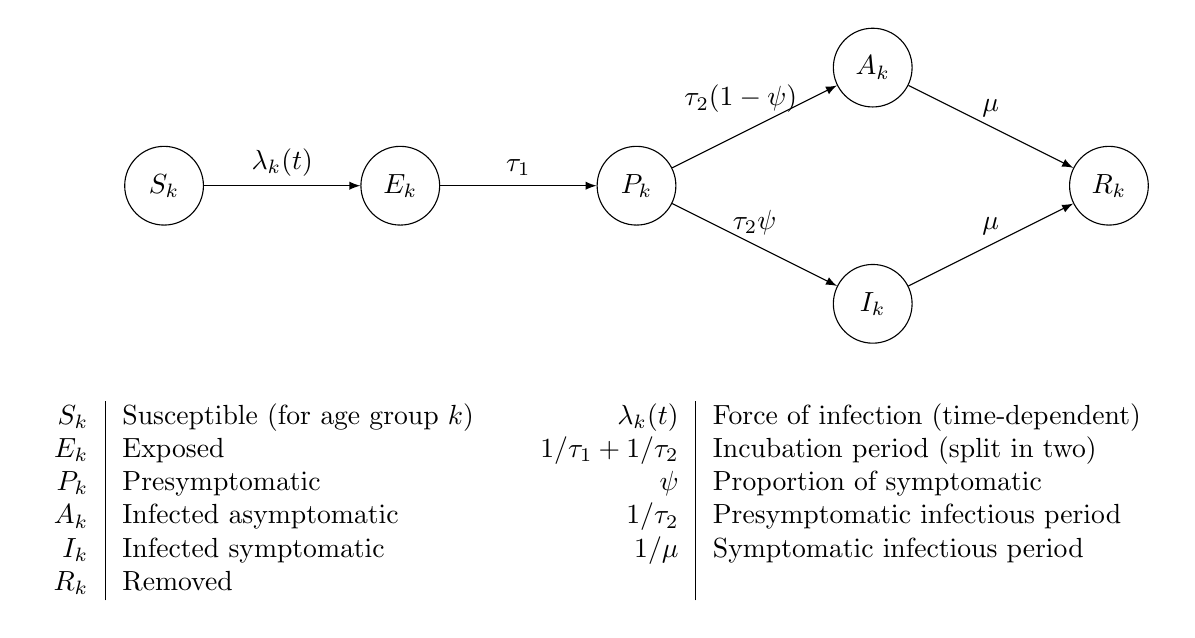
\begin{tikzpicture}
	 		% cascade of care
	 		\node[circle, draw, inner sep=0pt, minimum size=1cm] (S) at (0,0) {$S_k$};
	 		\node[circle, draw, inner sep=0pt, minimum size=1cm] (E) at (3,0) {$E_k$};
	 		\node[circle, draw, inner sep=0pt, minimum size=1cm] (P) at (6,0) {$P_k$};
%	 		\node[circle, draw, inner sep=0pt, minimum size=1cm,gray,dashed] (C) at (8.5,-2.5) {$C_k$};
%	 		\node[circle, draw, inner sep=0pt, minimum size=1cm,gray,dashed] (rho_C) at (12,-2.5) {$\rho_k C_k$};
	 		\node[circle, draw, inner sep=0pt, minimum size=1cm,fill=white] (I) at (9,-1.5) {$I_k$};
	 		\node[circle, draw, inner sep=0pt, minimum size=1cm] (A) at (9,1.5) {$A_k$};
	 		\node[circle, draw, inner sep=0pt, minimum size=1cm] (R) at (12,0) {$R_k$};
	 		
	 		\draw[->,>=latex] (S) edge node[above] { $\lambda_k(t)$} (E);
	 		\draw[->,>=latex] (E) edge node[above] { $\tau_1$ } (P);
	 		\draw[->,>=latex] (P) edge node[yshift=10,xshift=-5] { $\tau_2(1-\psi)$ } (A);
	 		\draw[->,>=latex] (P) edge node[above] { $\tau_2\psi$ } (I);
%	 		\draw[->,>=latex,gray,dashed] (P) edge[bend left=12] node[below] { $\tau_2\psi$ } (C);
	 		\draw[->,>=latex] (A) edge node[above] { $\mu$ } (R);
	 		\draw[->,>=latex] (I) edge node[above] { $\mu$ } (R);
%	 		\draw[double,gray] (C) -- node[above] { $\rho_k$ }  (rho_C);
%	 		
%	 		% legend
	 		\node (leg) at (5.5,-4) {
	 			\begin{tabular}{r|lp{0cm}r|l}
	 				$S_k$ & Susceptible (\alert{for age group $k$})& & $\lambda_k(t)$ & Force of infection (\alert{time-dependent})\\
	 				$E_k$ & Exposed & & $1/\tau_1+1/\tau_2$ & Incubation period (\alert{split in two})\\
	 				$P_k$ & Presymptomatic & &$\psi$ & Proportion of symptomatic \\	
	 				$A_k$ & Infected asymptomatic & & 	$1/\tau_2$ & Presymptomatic infectious period \\
	 				$I_k$ & Infected symptomatic& &	 $1/\mu$ & Symptomatic infectious period \\
	 				$R_k$ & Removed & & &\\% $\rho_k$ & Ascertainment proportion \\
	 			%	$C_k$ & Cumulative cases  & & $\rho_k C_k$ & Cumulative confirmed cases \\
	 		\end{tabular}};
	 	\end{tikzpicture}
 	}
 \end{figure}
}


\frame{
	\frametitle{Example}
	Posterior predictive check (Hubei):
		\begin{figure}
		\centering
		\includegraphics[width=1\linewidth]{example_hauser/supp_fit_16B.pdf}
	\end{figure}
	
}






\end{document}
